\subsection{Room}\label{Room}
The rooms are central parts of our game as they hold the information about who is where, and can thus be seen as the glue which keeps everything together. Our overall goal has been to be able to define a list of weathers for which we can then synthesize rooms which has these chosen weathers. In the meta language we can for instance define a list consisting of \textit{blizzard} and \textit{sunny}, and so the only two weather types which should be encountered in this variation are \textit{blizzard} and \textit{sunny}. We created in total four different weather effects, \textit{blizzard, sunny, night} and \textit{cloudy}. To make the room able to use different weathers we followed a strategy pattern where each weather type conforms to the \textit{IWeatherEffect} interface. Every time a player enters a room it will at random choose a weather effect from the defined possibilities, and its \textit{WeatherEffect} method is called. This way the room can conform to many different strategies as to how the weather should effect the player. \\
We found what makes a room to be what weather types it should be able to use, and whether there is a boss in the variation or not. Each of the weather effects have their own kinding which allows them to be either the weather or \textit{'none}. Given all weather type kindings has the type \textit{'none} in common, we only have to create a single combinator for this option as they can all share it. We can attempt to be a little more concrete by looking only at the semantic types in the following. We are looking for room. As mentioned this is defined by the weathers and whether there is a boss present or not. And so we are looking for: \textit{'bossActive(boss), 'weatherTypes(blizzardWeather, sunnyWeather, nightWeather, cloudyWeather) $\to$ room(blizzardWeather, sunnyWeather, nightWeather, cloudyWeather, boss)}. We read this as we need something of semantic type \textit{'bossActive} intersected by the kinding \textit{boss} and we need something of semantic type \textit{weatherTypes} intersected by the weather kindings to get something of semantic type \textit{'room} intersected by the weather type and boss kindings. The boss part is fairly straightforward as either there is a boss or not. The kinding is reused from the player and the combinator for when the boss is present consists of three methods which are added to the room, whereas if the boss is not present, the combinator is an empty string. The two combinators for \textit{'weatherTypes} are more complex. We have two as the code needed for having no weather effects and having one or more weathers are quite distinct.

\begin{figure}[H]
	\centering
	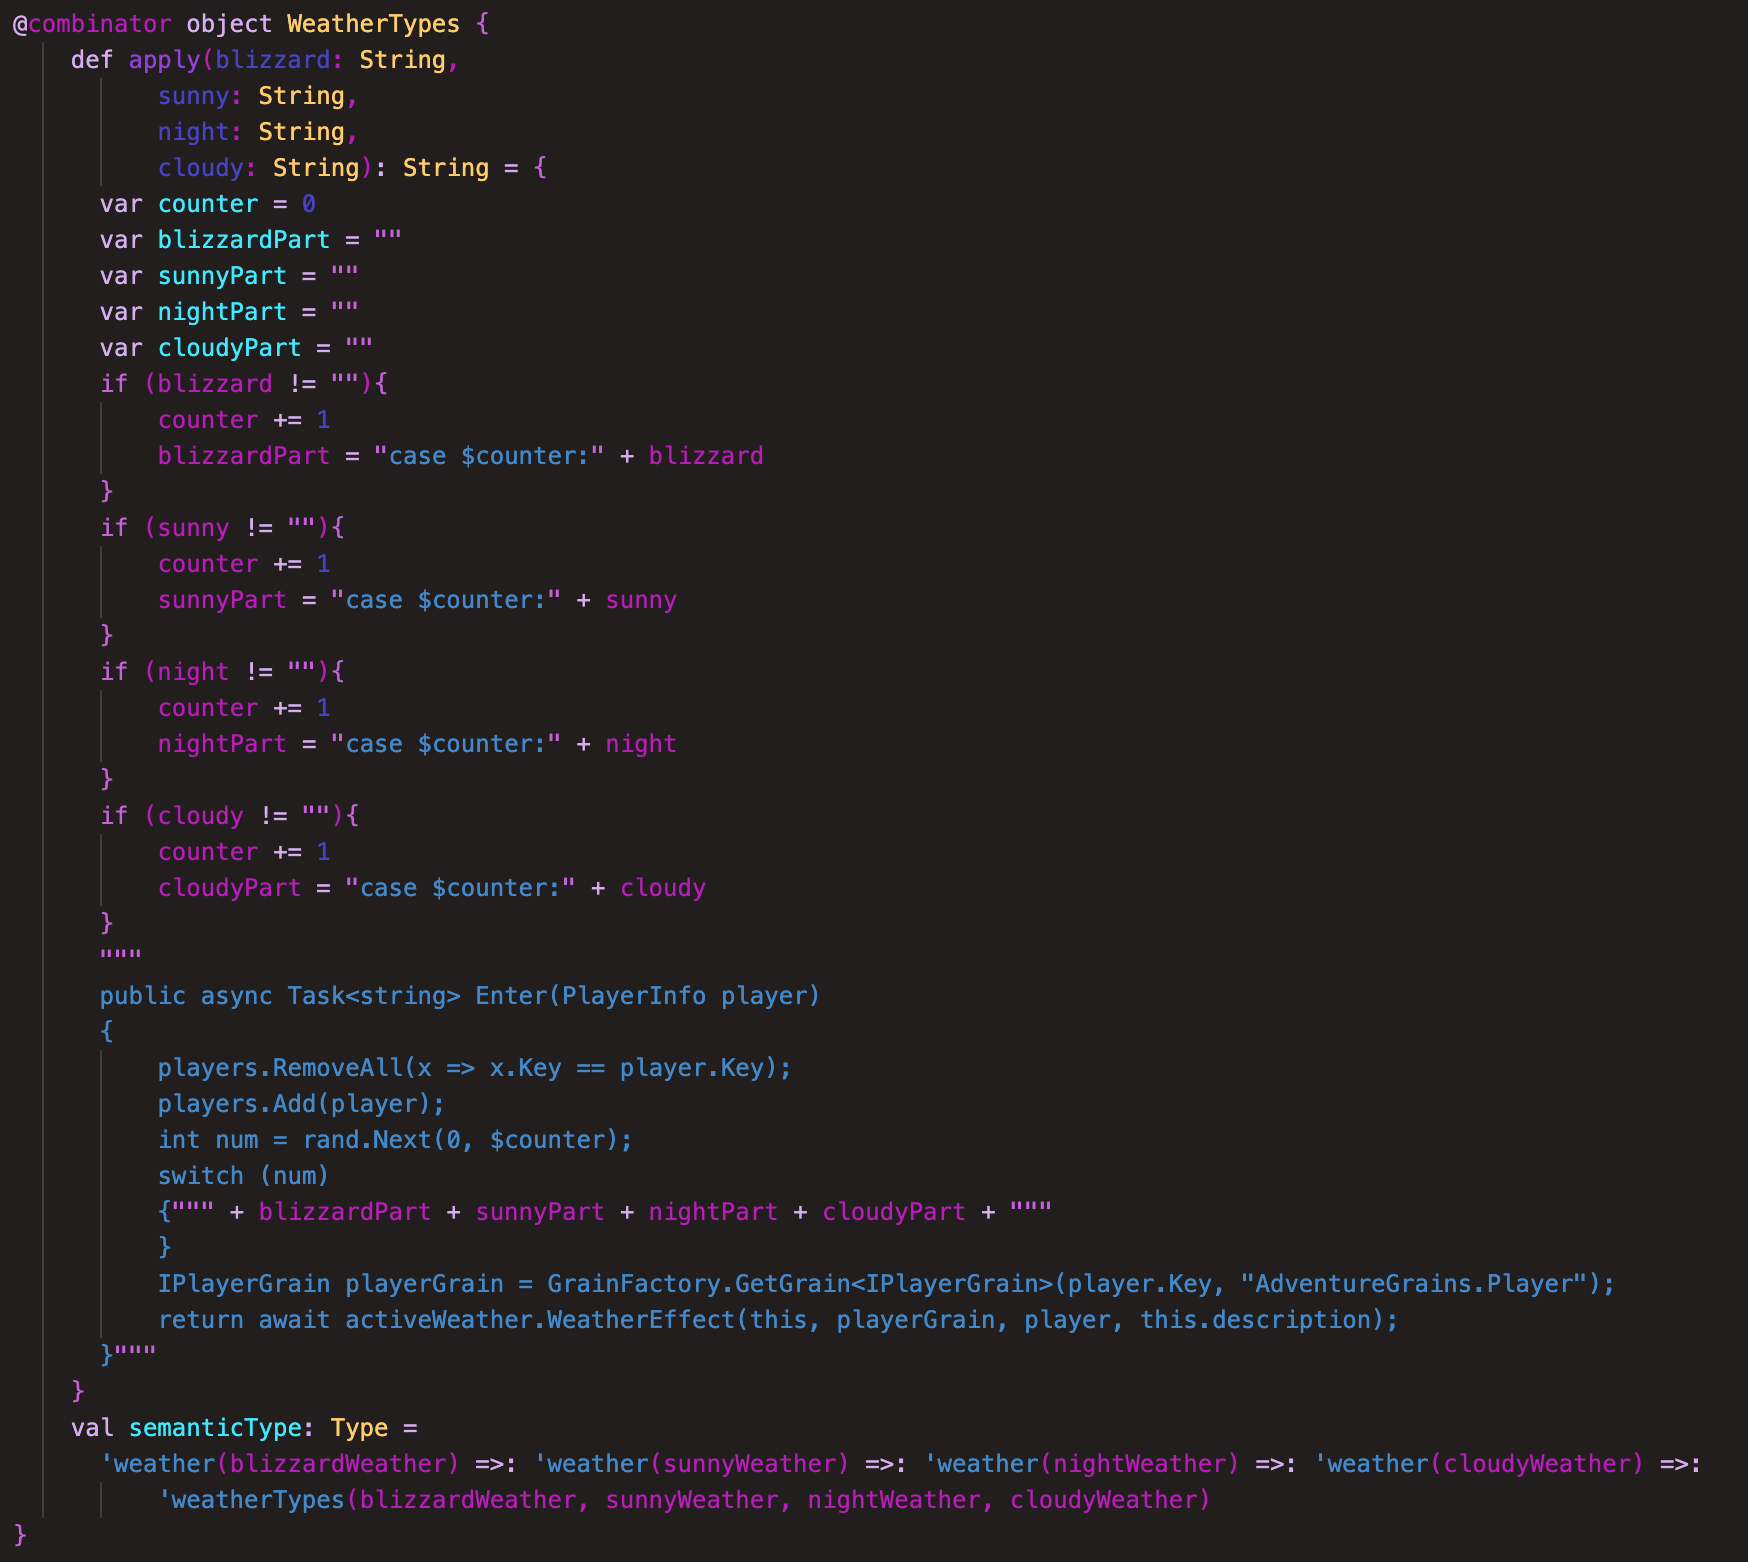
\includegraphics[width=\linewidth]{Materials/Decomposition/Room/WeatherEffects}
	\caption{The combinator used to create variations with weather effects.}
	\label{WeatherEffects}
\end{figure}
In \autoref{WeatherEffects} we see the combinator for creating weather effects. As it is not trivial how this combinator works we will go a little more into detail about how it. The overall structure we are working towards is a switch case where we at random will choose what weather effect the player should experience. We see that we need four \textit{'weather} types, one for each possible weather effect. These come from simple combinators providing two lines of code for the \textit{WeatherTypes} combinator (seen in \autoref{WeatherEffects}). We then check each of the weathers if they should be present by checking whether the string provided to \textit{WeatherTypes} is empty or not. If it is not empty, the code provided it appended to "case " and the number of a counter. If two weathers are present, the first will then be of case 0, and the second of case 1. After we have created the cases for each of the weathers present, we then insert them in the 'static' part of the combinator as part of the switch statement. We note that this combinator ends by calling a weather effects \textit{WeatherEffect} method. All the weathers call the room's \textit{Description} method which is the biggest change when looking at the combinator used when we do not have any weather effects, as now the room has to make this call itself. The combinator for no weather effects can be seen in \autoref{NoneWeather}.

\begin{figure}[H]
	\centering
	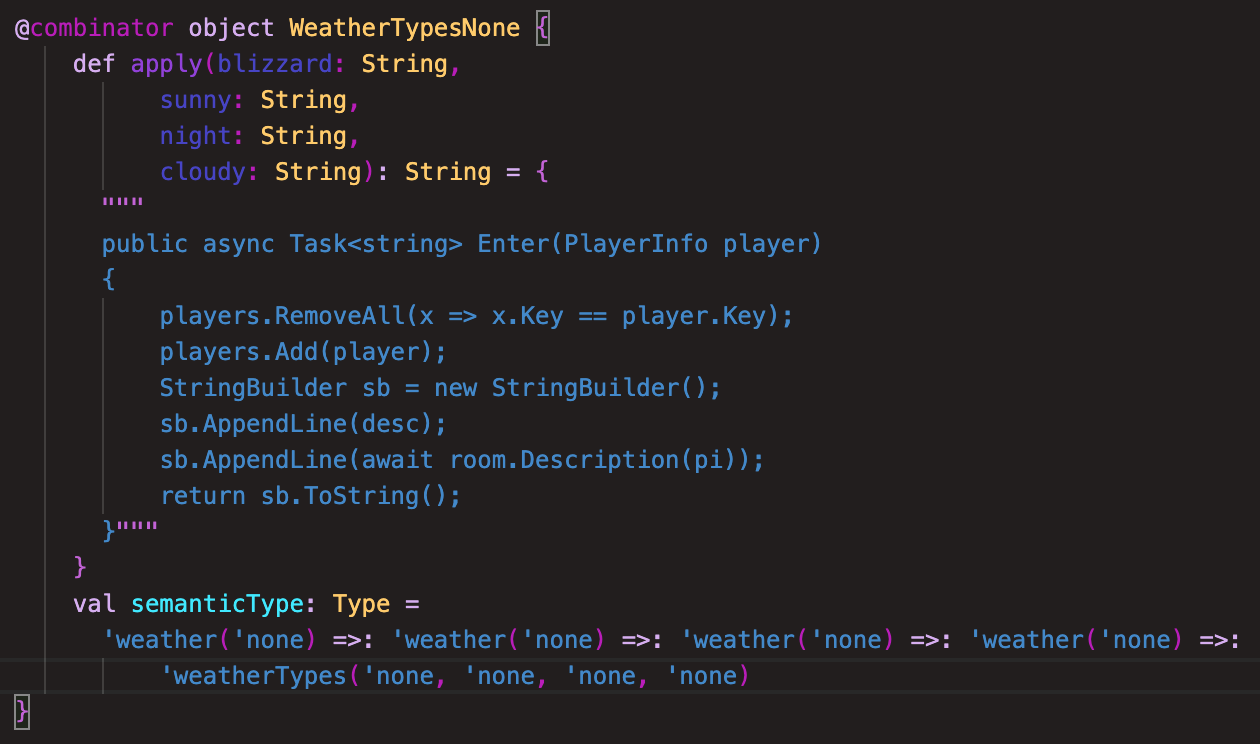
\includegraphics[width=\linewidth]{Materials/Decomposition/Room/NoneWeather}
	\caption{The combinator used to when we do not want weather effects.}
	\label{NoneWeather}
\end{figure}
Unfortunately we see that when we create a variation with no weather effects we will get two variations. This is because both combinators accepts four \textit{'weather} types intersected by \textit{'none}. We could avoid this issue by intersecting \textit{'room} further. For instance adding a kinding \textit{'weatherPresent'} which can take the values \textit{'weatherIsPresent} and \textit{'weatherIsNotPresent}. We could then add a combinator which provides the first few lines which \textit{WeatherTypes} and \textit{WeatherTypesNone} (seen in \autoref{NoneWeather}) has in common and has the semantic type \textit{weatherEffect(weatherPresent)}. \textit{WeatherTypes} would then require \textit{weatherEffect(weatherIsPresent)} and \textit{WeatherTypesNone} would require \textit{weatherEffect(weatherIsNotPresent)}. Then the \textit{weatherPresent} kinding would be set in the \textit{SemanticRoomTarget} method depending on whether all weather kindings are \textit{'none} or not. This is however, a lot of additional complexity and begs the question, is creating a combinator for the first few common lines of code meaningful? The consequence of not doing this, is the developer needs to choose the correct variation of the room, which we do not see as a huge issue. And we thus value the simpler solution more, as we see the added complexity to do more harm than having to choose between two variations do. However, this is a small project, and in a bigger setting it might be better to choose the alternative solution as it is more scalable.\\

As we now can synthesize code based on defined parameters in the metalanguage, we conclude we have successfully synthesized the room, and we have met all of the goals we formulated as our driving forces.

